\documentclass[12pt]{article}

% Packages
\usepackage{graphicx}
\usepackage{geometry} 
\usepackage{titlesec} 
\usepackage{fancyhdr} 
\usepackage{hyperref} 
\usepackage{float}

% Page setup
\geometry{a4paper, margin=1in}
\pagestyle{fancy}
\fancyhf{}
\fancyhead[R]{RTGP Project Report}
\fancyfoot[C]{\thepage}

\titleformat{\section}
{\normalfont\Large\bfseries}{\thesection}{1em}{}
\titleformat{\subsection}
{\normalfont\large\bfseries}{\thesubsection}{1em}{}

% Begin document
\begin{document}

% Title
\begin{titlepage}
    \centering
    \vspace*{2cm}
    {\Huge\bfseries Real Time Graphics Programming Project Report\par}
    \vspace{1.5cm}
    {\Large\itshape Compagnoni Alessandro\par}
    \vspace{0.5cm}
   {\large UNIMI A.A. 2023/2024\par}
    \vfill
    
\includegraphics[width=0.8\textwidth]{Images/logoUnimi.png} 
    \vfill
\end{titlepage}

% Table of Contents
\tableofcontents
\newpage

% Sections
\section{Overview}
\label{sec:overview}

This project implements a 3D environment using OpenGL, allowing users to navigate within 3 square rooms. Inside the rooms various 3D objects are placed, each rendered with a different material based on shaders that showcase various types of noise with different parameters, all freely adjustable by the user thanks to the dedicated UI.

\section{Design Choices}
\label{sec:project_details}
\subsection{Technologies}
The following technologies were selected to ensure efficient rendering, cross-platform compatibility, and streamlined development for the project:

\begin{itemize}
\item OpenGL Version 3.3+:
\newline
OpenGL's modern shader-based architecture was chosen to leverage direct control over vertex and fragment processing. By utilizing GLSL shaders, the pipeline enables complex procedural effects while maintaining high performance.

\item GLFW (Graphics Library Framework):
\newline
GLFW provides robust window management and input handling, ensuring consistent behavior across operating systems, also its event-driven architecture simplifies interaction with user inputs.

\item GLM (OpenGL Mathematics):
\newline
GLM mathematics library is optimized for graphics programming. It offers essential data types (e.g., vectors, matrices) and prebuilt functions for common transformations (e.g., translation, projection).

\item ImGui:
\newline
ImGui is a graphical user interface library for C++. It is simple, fast and portable and allows fast iteration and implementation of creation tools and visualization / debug tools.
\end{itemize}

\subsection {Organization}
The project is organized as follows:
\begin{itemize}
\item C++ file containing the code with the main function and all other functions called "Rooms.cpp", this file is located in the "src" directory.
\item Directory called "shaders" containing all the fragment.glsl and vertex.glsl shader files for each of the materials used in the project.
\item All the necessary dependencies and library located in the "include", "imgui" and "lib" directories.
\end{itemize}

\newpage

\subsection{Architecture}
The scene is organized in 3 different square rooms, where each of the walls, floor and ceiling material's are based on a different shader: the walls' shader is made to make them look like wooden walls, while the ceiling and floor utilize a marble-like shader. The rooms are connected by 2 short corridors that utilize a dark-grey colored shader to appear neutral.

\begin{figure}[H]
    \centering
    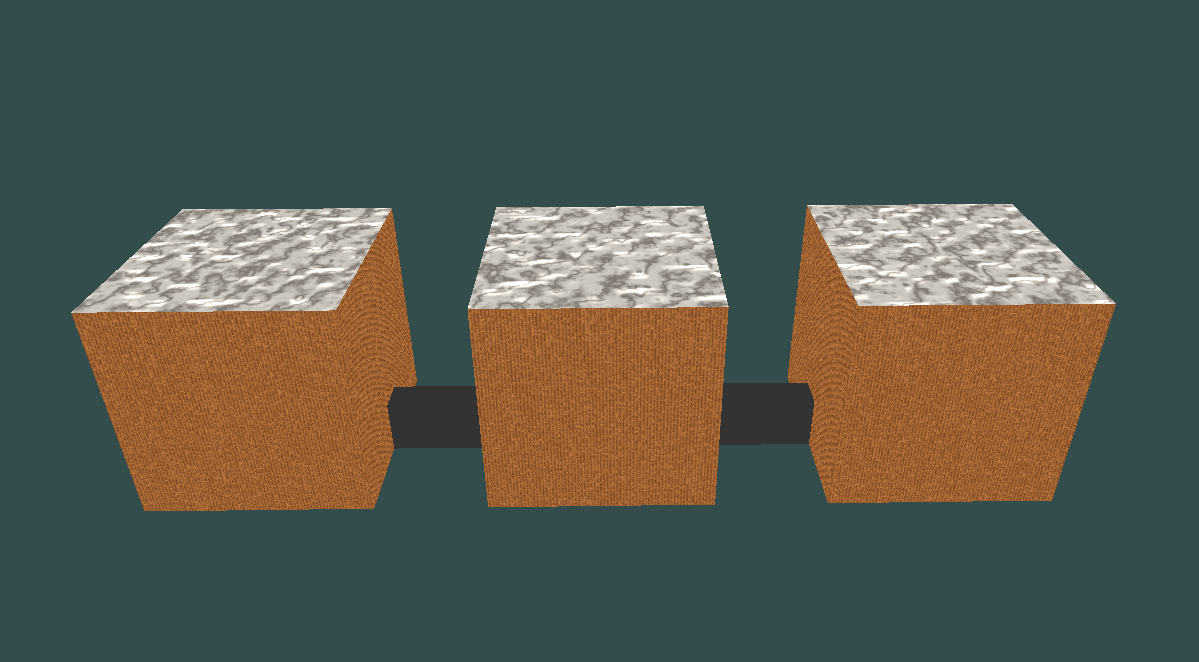
\includegraphics[width=0.8\textwidth]{Images/architecture.png}
    \caption{Structure and architecture of the 3D space as seen from the outside}
\end{figure}

Inside each of the first 2 rooms we can find 3 objects (a sphere, a pyramid and a cube), while in the last room we only find 2 objects of larger dimensions (a sphere and a cube). 

\begin{figure}[H]
    \centering
    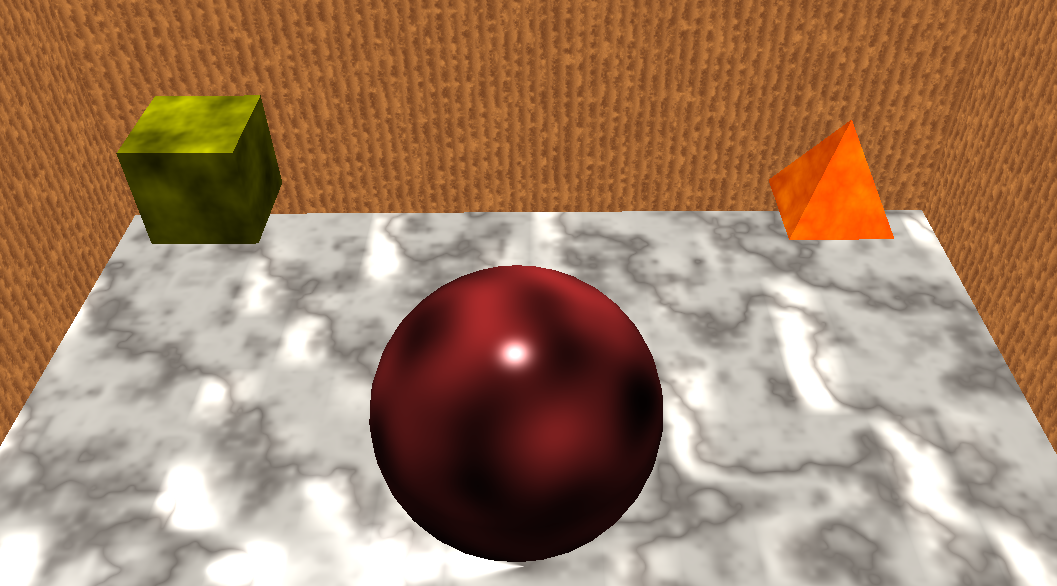
\includegraphics[width=0.8\textwidth]{Images/firstRoom.png}
    \caption{First room}
\end{figure}

\begin{figure}[H]
    \centering
    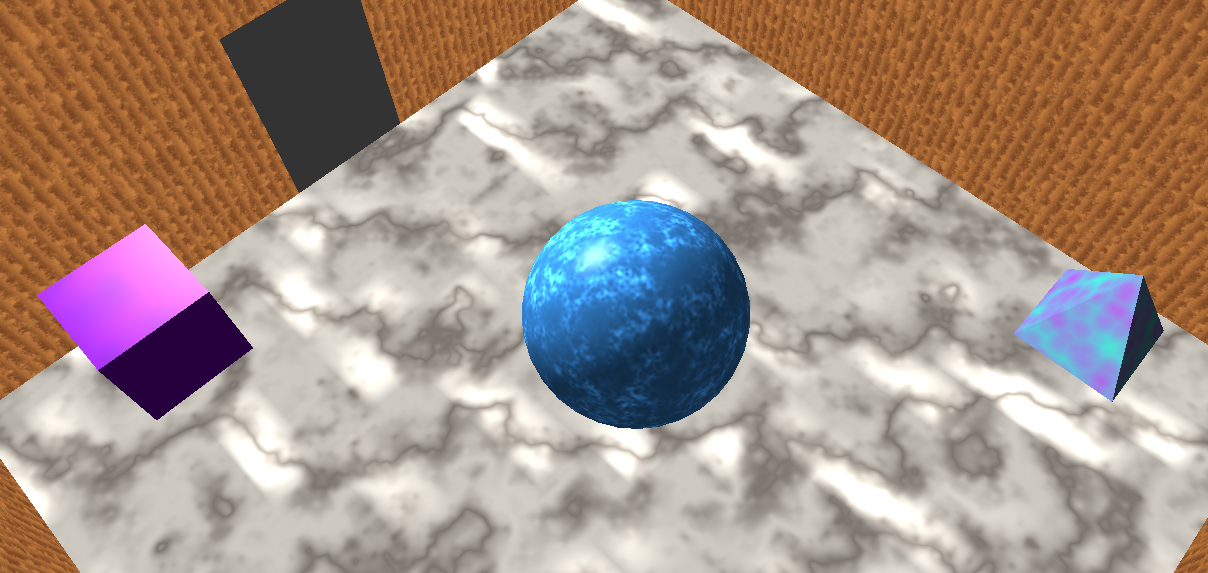
\includegraphics[width=0.8\textwidth]{Images/secondRoom.png}
    \caption{Second room}
\end{figure}

\begin{figure}[H]
    \centering
    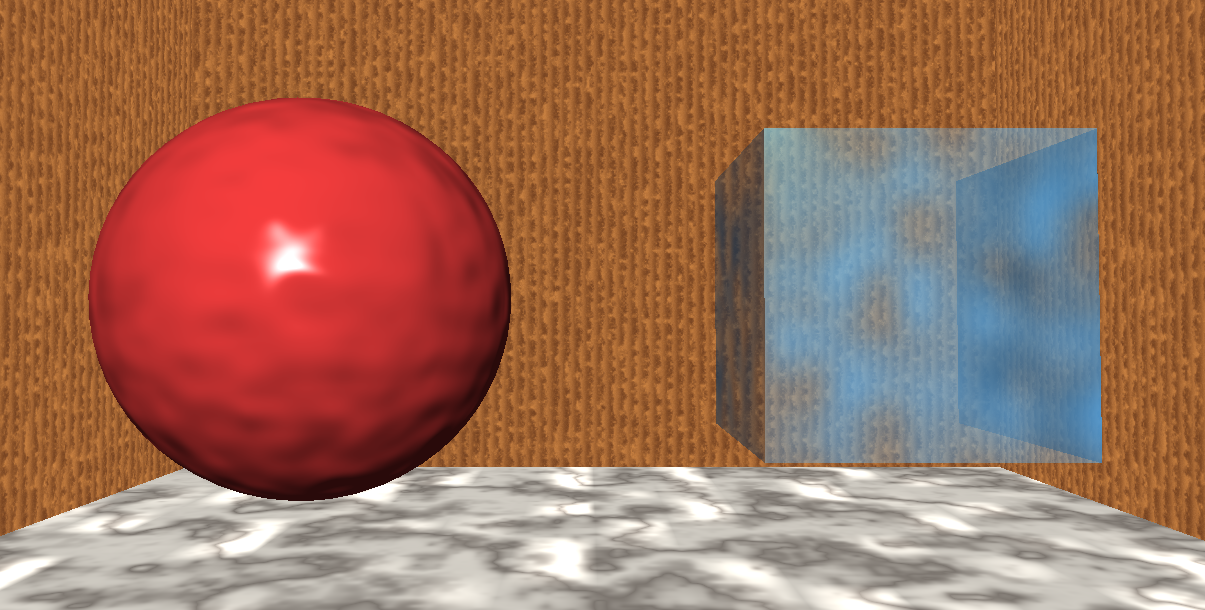
\includegraphics[width=0.8\textwidth]{Images/thirdRoom.png}
    \caption{Third room}
\end{figure}
\subsection {Controls}
The user is able to move and look around in this space by using the WASD keys to move and the mouse to orient the camera. 

\newpage

\section{Algorithms and Techniques}
\label{sec:algorithms}
This section will explain in detail all types of noise utilized and where the user can find them in the project.
\subsection {Noises}

\newpage

\section{Implementation Details}
\label{sec:implementation}

\newpage

\section{Performance Evaluation}
\label{sec:performance}

\end{document}